\documentclass[a4paper,10pt]{article}
\usepackage[utf8]{inputenc}
\usepackage[margin=1.5cm]{geometry}
\usepackage{enumitem}
\usepackage{hyperref}
\usepackage{xcolor}
\usepackage{graphicx}
\usepackage{xltxtra}
\usepackage{fontspec}
\usepackage{titlesec}
\usepackage{ulem}
% \setmainfont{Times New Roman}  % 기본 영문 폰트 설정

\newfontfamily\hangulfont{NanumSquare}  % 한글 폰트 설정

\titleformat{\section}
  {\normalfont\large\bfseries}{}{0em}{}[{\titlerule[0.8pt]}]
  
\titlespacing*{\section}{0pt}{12pt}{6pt}
\setlist[itemize]{leftmargin=15pt,      %
                    labelindent=16pt,   %
                    itemindent=-5pt,    % item과 글자 사이 간격
                    labelsep=5pt,       %
                    itemsep=0pt,        %item 항목 간격
                    parsep=3pt          %item 내부 간격
}
\setlist[itemize,2]{topsep=-3pt,
                    leftmargin=0pt,      %
                    labelindent=0pt,   %
                    itemindent=0pt,    % item과 글자 사이 간격
                    labelsep=0pt,       %
                    itemsep=0pt,        %item 항목 간격
                    parsep=0pt          %item 내부 간격
}

\begin{document}

\noindent
\begin{minipage}[c]{0.7\textwidth}
    \LARGE\textbf{Jangseop Park} \large ({\hangulfont \textbf{박장섭}}) \vspace{2mm}\\
    \normalsize \textbf{Ph.D. Candidate}, Cho Chun Shik Graduate School of Mobility, KAIST \\
    \begin{minipage}{\linewidth}
    \vspace{5pt}
    \hspace{10pt}Room F431, 193 Munji-ro, Yuseong-gu, Daejeon, 34051, Republic of Korea
    \end{minipage}
    \begin{minipage}{\linewidth}
    \vspace{2pt}
    \hspace{10pt}\textbf{E-mail:} \href{mailto:jangseop@kaist.ac.kr}{\textcolor{blue}{jangseop@kaist.ac.kr}}\hspace{65pt} \textbf{Homepage:} \href{https://jangseop.page}{\textcolor{blue}{jangseop.page}}
    \end{minipage}
\end{minipage}
\hfill
\begin{minipage}[c]{0.165\textwidth}
    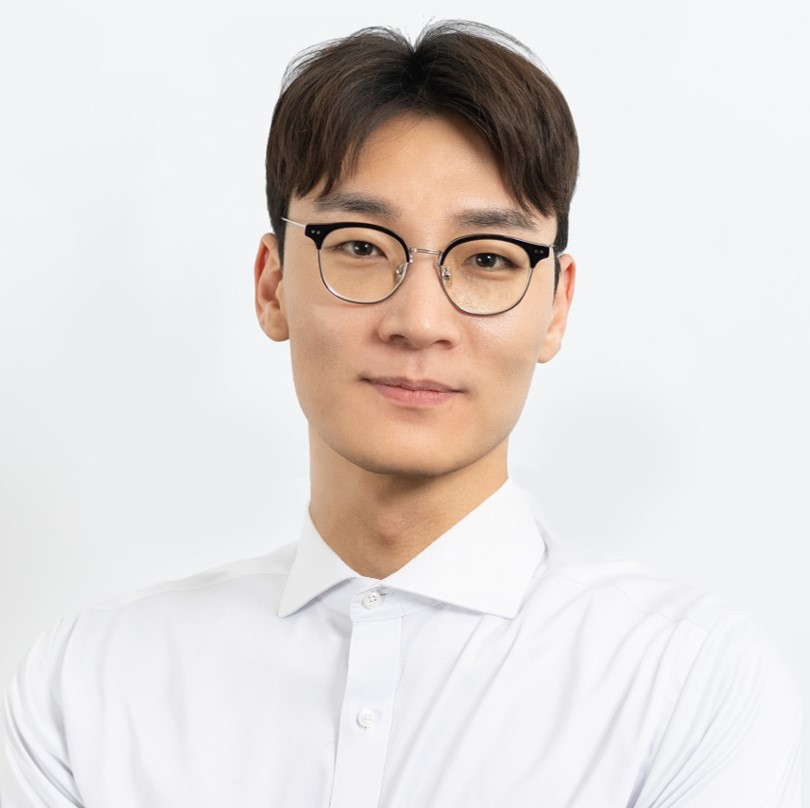
\includegraphics[width=\linewidth]{profile.jpg} % 프로필 이미지 삽입
\end{minipage}

\section*{EDUCATION}
\begin{itemize}[left=0pt]
    \item \textbf{Korea Advanced Institute of Science and Technology (KAIST)}   \hfill \textit{\textcolor{gray}{Daejeon, Korea}} \\
    \textbf{Ph.D. Candidate.} CCS Graduate School of Mobility                   \hfill Mar. 2023 - Feb. 2027 \\
    \textbf{M.S.} CCS Graduate School of Mobility                               \hfill Aug. 2020 - Feb. 2023 \\
    \begin{minipage}{\linewidth}
    \hspace{5pt}Advisor: Prof. Namwoo Kang, (\textbf{Homepage}: \href{https://www.smartdesignlab.org/}{\textcolor{blue}{smartdesignlab.org}})
    \end{minipage}
    \item \textbf{Korea University of Technology and Education}                 \hfill \textit{\textcolor{gray}{Cheonan, Korea}} \\
    \textbf{B.S.} Mechatronics Engineering                                      \hfill Feb. 2012 - Aug. 2019
\end{itemize}

\section*{EXPERIENCE}
\begin{itemize}[left=0pt]
\item \textbf{Graduate Researcher}                                              \hfill \textit{\textcolor{gray}{Daejeon, Korea}} \\
    Smart Design Lab., KAIST                                                    \hfill Sep. 2020 - Present
\item \textbf{AI Researcher}                                                    \hfill \textit{\textcolor{gray}{Daejeon, Korea}} \\
    Narnia Labs                                                                 \hfill Feb. 2023 - Aug. 2024
\item \textbf{Mechanical Design Engineer}                                       \hfill \textit{\textcolor{gray}{Incheon, Korea}} \\
    ATI | Advanced Technology Inc.                                              \hfill May. 2019 - Oct. 2019
\item \textbf{Student Researcher}                                               \hfill \textit{\textcolor{gray}{Cheonan, Korea}} \\
    Computer-Aided-Engineering Lab., KOREATECH                                  \hfill Apr. 2017 - Dec. 2018
\end{itemize}

\section*{INDUSTRIAL PROJECTS}
\begin{itemize}[left=0pt]
    \item \textbf{Samsung Heavy Industries}
    \begin{itemize}
        \item[] Generative AI-Based Sloshing Load Prediction and CCS Configuration Optimization    \hfill Apr. 2026 - Oct. 2026
    \end{itemize}
    \item \textbf{Hyundai Motor Group}
    \begin{itemize}
        \item[] Development of a Battery Failure Prediction Algorithm Based on Anomaly Detection   \hfill Feb. 2024 - Mar. 2025
        \item[] Development of a GNN-Based Deep Learning Library for Collision Analysis Prediction \hfill Sep. 2023 - Dec. 2023
        \item[] GNN-Based Deep Learning for Performance Prediction from 3D Geometry Data           \hfill Jul. 2022 - Jun. 2023
        \item[] Generative Design Guidelines and AI-Based Classification for Automotive Road Wheels \hfill Jul. 2021 - Jul. 2022
    \end{itemize}
    \item \textbf{LG Display}
    \begin{itemize}
        \item[] Optimization of Panel Layered Structures Using Generative Design and MeshGraphNet  \hfill May. 2022 - Feb. 2023
    \end{itemize}
    \item \textbf{Korea Expressway Corporation}
    \begin{itemize}
        \item[] Development of an Expressway Accident Risk Index for Identifying Hotspots          \hfill Mar. 2021 - Dec. 2021
    \end{itemize}
    \item \textbf{Korea Railroad Corporation (KORAIL)}
    \begin{itemize}
        \item[] Transportation Performance Analysis and Modal Substitutability under COVID-19      \hfill Sep. 2020 - Feb. 2021
    \end{itemize}
\end{itemize}


\section*{PUBLICATIONS}
\begin{itemize}[left=0pt]
    \item \textbf{Park, J.}, \& Kang, N.* (2026). “AutoATC: Automated Analytical Target Cascading Decomposition with LLM-Based Multi-Agent System." (Under review)

    \item \textbf{Park, J.}, \& Kang, N.* (2026). “LLM-Guided Adaptive Penalty Parameter Updates for Analytical Target Cascading." (Under review)

    \item \textbf{Park, J.}, \& Kang, N.* (2026). “Point-DeepONet: Predicting Nonlinear Fields on Non-Parametric Geometries under Variable Load Conditions." \textit{Neural Networks, 108560}. \href{https://drive.google.com/file/d/1lhtuo7lj0tQHgUiy_O5BtJQ1Z8Z5uwCw/view?usp=sharing}{\textcolor{blue}{(PDF)}} \href{https://github.com/jangseop-park/Point-DeepONet}{\textcolor{blue}{(code)}} \href{https://www.kaggle.com/datasets/jangseop/point-deeponet-dataset}{\textcolor{blue}{(dataset)}}

    \item Kim, J., \textbf{Park, J.}, Kim, N., Yu, Y., Chang, K., Woo, C. S., Yang, S.*, \& Kang, N.* (2025). “Physics-Constrained Graph Neural Networks for Spatio-Temporal Prediction of Drop Impact on OLED Display Panels." \textit{Expert Systems with Applications, 126907}. \href{https://drive.google.com/file/d/19UGsFCe5Sy11yK7XyVSx3SH4UjWmDPvP/view?usp=drive_link}{\textcolor{blue}{(PDF)}}

    \item Hong, S., Kwon, Y., Shin, D., \textbf{Park, J.}, \& Kang, N.* (2025). “DeepJEB: 3D Deep Learning-Based Synthetic Jet Engine Bracket Dataset." \textit{Journal of Mechanical Design, 147(4)}. \href{https://drive.google.com/file/d/17VQTiKB6QXh4zt8W-lwTEPPdEV8HCR40/view?usp=sharing}{\textcolor{blue}{(PDF)}}  \href{https://www.narnia.ai/dataset}{\textcolor{blue}{(dataset)}}

    \item \textbf{Park, J.}, \& Kang, N. (2024). “BMO-GNN: Bayesian Mesh Optimization for Graph Neural Networks to Enhance Engineering Performance Prediction." \textit{Journal of Computational Design and Engineering, 11(6), 260-271}. \href{https://drive.google.com/file/d/1aM3jgCQOcru5nmoYqRsTlN6fyfdzqllY/view?usp=sharing}{\textcolor{blue}{(PDF)}}

    \item Yun, J., Lee, J., \textbf{Park, J.}, Chung, K., \& Lee, J.* (2022). “How to Measure the Network Vulnerability of Cities to Wildfires: Cases in California, USA." \textit{Transportation research record, 2676(12), 382-395}. \href{https://drive.google.com/file/d/1KfCyHU_KTTuBgNK6t3dWyKFuCxVgSrAu/view?usp=sharing}{\textcolor{blue}{(PDF)}}
\end{itemize}

\section*{INTERNATIONAL CONFERENCES}
\begin{itemize}[left=0pt]
    \item \textbf{Park, J.}, \& Kang, N.* (2026). “LLM-Guided Adaptive Penalty Parameter Updates for Analytical Target Cascading”, In \textit{Asian Congress of Structural and Multidisciplinary Optimization (ACSMO 2026)}.

    \item \textbf{Park, J.}, \& Kang, N.* (2025). “A PointNet-Enhanced Operator Network for Nonlinear Analysis of Non-Parametric 3D Geometries Under Varying Load Conditions”, In \textit{16th World Congress of Structural and Multidisciplinary Optimisation (WCSMO 16)}.

    \item Kim, J., \textbf{Park, J.}, Yang, S., \& Kang, N.* (2024). “Design Optimization of Multi-layered Display Panels for Drop Impact using Physics-Constrained Graph Neural Network”, \textit{The 26th International Congress of Theoretical and Applied Mechanics 2024 (ICTAM2024)}.
    
    \item \textbf{Park, J.}, \& Kang, N.* (2023). “Bayesian Mesh Optimization for Graph Neural Networks to Enhance Engineering Performance Prediction”, In \textit{ASME 2023 International Design Engineering Technical Conferences \& Computers and Information in Engineering Conference (IDETC/CIE 2023)}.
    
    \item \textbf{Park, J.}, \& Kang, N.* (2023). “How to Apply AI to Real-World Design Problems", In \textit{ASME 2023 International Design Engineering Technical Conferences \& Computers and Information in Engineering Conference (IDETC/CIE 2023)}.
    
    \item Yun, J., Lee, J.Y., \textbf{Park, J.}, Chung, K., and Lee, J.* (2022), “How to Measure the Vulnerability of Cities to Wildfires: Cases in California", \textit{Transportation Research Board (TRB) 101st Annual Meeting}.
\end{itemize}

\section*{DOMESTIC CONFERENCES}
\begin{itemize}[left=0pt]
    \item Cho, Y., \textbf{Park, J.}, \& Kang, N.* (2026). “A Data-Driven Framework for Railway Track Condition Assessment Using the Analytic Hierarchy Process", In \textit{The Korean Society of Mechanical Engineers (KSME)}.

    \item \textbf{Park, J.}, \& Kang, N.* (2025). “DialogCAD: Interactive CAD Generation Framework with a Multi-Agent System via Model Context Protocol", In \textit{The Korean Society of Mechanical Engineers (KSME)}.

    \item \textbf{Park, J.}, Kim, J., Jang, W., Lee, Y., Lee, S., \& Kang, N.* (2025). “A Study on 3D Topology Optimization Shape Reconstruction with CSG-Based Deep Learning", In \textit{The Korean Society of Mechanical Engineers (KSME)}.

    \item \textbf{Park, J.}, \& Kang, N.* (2025). “SG-DeepONet: A Spatial Gradient-Aware Deep Operator Network for Pressure and Shear Stress Prediction in Vehicle Aerodynamic Analysis", In \textit{The Korean Society of Mechanical Engineers (KSME)}.
    
    \item \textbf{Park, J.}, \& Kang, N.* (2024). “Stress Field Prediction in Nonlinear Static Analysis for Arbitrary 3D Geometries Using Latent-DeepONet", In \textit{The Korean Society of Mechanical Engineers (KSME)}.
    
    \item Hong, S., Kwon, Y., Shin, D., \textbf{Park, J.}, and Kang, N.* (2024). “DeepJEB: 3D Deep Learning-based Synthetic Jet Engine Bracket Dataset”, In \textit{The Korean Society of Mechanical Engineers (KSME)}.
    
    \item Shin, D., \textbf{Park, J.}, Seo, M., \& Kang, N.* (2024). “3D Field Prediction and Uncertainty Quantification with Implicit Neural Representation", In \textit{The Korean Society of Mechanical Engineers (KSME), 289-290}.
    
    \item \textbf{Park, J.}, Kim, J., Yu, Y., Kim, N., Ha, S., Jang, K., \& Kang, N.* (2023). “A Study on Impact Analysis based on Graph Neural Networks for Optimization of the Display Panel Structure", In \textit{The Korean Society of Mechanical Engineers (KSME), 144-145}.
    
    \item \textbf{Park, J.}, \& Kang, N.* (2022). “Bayesian Mesh Optimization for Graph Neural Networks", In \textit{The Korean Society of Mechanical Engineers (KSME), 1626-1628}.
    
    \item \textbf{Park, J.}, Shin, D., Yoo, S., \& Kang, N.* (2022). “Preliminary Study on 3D Wheel Performance Prediction Using Graph Neural Networks", In \textit{The Korean Society of Mechanical Engineers (KSME), 316-317}. (Best Paper)
    
    \item Yun, J., Lee, J., \textbf{Park, J.}, Chung, K., \& Lee, J.* (2021). “How to Measure the Vulnerability of Cities to Wildfires, Cases in California", In \textit{Korean Society of Transportation, 436-437}.
    
    \item Mok, H, \textbf{Park, J.}, Lee, J., Han, D., \& Kim, D.* (2021). “Development of Express Accident Risk Index (ex-ARI) for Identifying Hotspots", In \textit{The Korean Society of Civil Engineers (KSCE), 57-58}.
    
    \item Mok, H., Lee, J., Han, D., \textbf{Park, J.}, \& Kim, D.* (2021). “Establishment of Traffic Safety Measures based on Accident Risk Idex(ex-ARI), Cases in Dangjin Yeongdeok Expressway", In \textit{The the Korean Society of Civil Engineers (KSCE), 506-507}.
    
    \item \textbf{Park, J.}, Kim, D., Mok, H., Han, D., \& Lee, J.* (2021). “Identifying Fatal and Severe Accident Hotspots based on Multiple Safety Performance Measures", In \textit{The Korean Society of Civil Engineers (KSCE), 49-50}. (Best Paper)
\end{itemize}

\section*{AWARDS}
\begin{itemize}[left=0pt]
    \item \textbf{Best Presentation Award}, Korean Society of Mechanical Engineers \hfill May 2022
    \item \textbf{Best Presentation Award}, Korean Society of Civil Engineering \hfill Nov 2021
    \item \textbf{Best Poster Award}, Korean Society of Civil Engineering \hfill Nov 2021
    \item \textbf{Minister of Science, Technology \& Telecommunication Award}, Capstone Design Fair \hfill Oct 2018
    \item \textbf{Korea Institute for Robot Industry Advancement Award}, SEOULTECH Robot Competition \hfill Oct 2018
    \item \textbf{Chancellor’s Award, Kyungnam University}, Changwon National Robot Competition \hfill Sep 2018
    \item \textbf{KOREATECH Industrial-Academic Cooperation Award}, SolidWorks Technology Competition \hfill Dec 2017
    \item \textbf{Chancellor’s Award, KOREATECH}, University Engineering Design Contest \hfill Nov 2017
\end{itemize}


\section*{OTHERS}
\begin{itemize}[left=0pt]
    \item \textbf{TA}, KAIST MO833 Lecture: "AI-based Mobility Design", Overview of DeepONet Applications \hfill Nov. 2024
    \item \textbf{TA}, KAIST MO833 Lecture: "AI-based Mobility Design" \hfill Mar. 2024 - Jun. 2024
    \item \textbf{TA}, KAIST Industry-Academic Collaboration Lecture: "Analysis Prediction to Optimization with AI" \hfill Feb 2024
    \item \textbf{Patent}, Apparatus and Method for Interactive CAD Generation Based on \hfill May 2025 \\
    a Multi-Agent System via a Model Context Protocol, KR 10-2025-0091992
    \item \textbf{Patent}, Wheelchair Maneuverability Enhancement, KR 10-2018-0015617 \hfill Feb 2018
\end{itemize}

\end{document}
